% use paper, or submit
% use 11 pt (preferred), 12 pt, or 10 pt only

%\documentclass[letterpaper, preprint, paper,11pt]{AAS}	% for preprint proceedings
\documentclass[letterpaper, paper,11pt]{AAS}		% for final proceedings (20-page limit)
%\documentclass[letterpaper, paper,12pt]{AAS}		% for final proceedings (20-page limit)
%\documentclass[letterpaper, paper,10pt]{AAS}		% for final proceedings (20-page limit)
%\documentclass[letterpaper, submit]{AAS}			% to submit to JAS

\usepackage{AAS_packages}
%\usepackage{subfigure} % have subcaption in use instead
%\usepackage[notref,notcite]{showkeys}  % use this to temporarily show labels

\PaperNumber{XX-XXX}

\begin{document}

\title{Geometric Control for Autonomous Landing on Asteroids}

\author{Shankar Kulumani and Taeyoung Lee\thanks{Mechanical and Aerospace Engineering, George Washington University, 800 22nd St NW, Washington, DC 20052, Tel: 202-994-8710, Email: \href{mailto:skulumani@gwu.edu}{\{skulumani,tylee\}@gwu.edu}.}
}


\maketitle{} 		

\begin{abstract}
    This paper considers the coupled orbit and attitude dynamics of a dumbbell spacecraft around an asteroid. 
    Geometric methods are used to derive the coupled equations of motion, defined on the configuration space \(\SE\), and then a nonlinear controller is designed to enable trajectory tracking of desired landing trajectories.
    Rather than relying on sliding mode control or optimization based methods, the proposed approach avoids the increased control utilization and computational complexity inherent in other techniques.
    The nonlinear controller is used to track a desired landing trajectory to the asteroid surface. 
    A monocular imaging sensor is used to provide position and attitude estimates using visual odometry to enable closed-loop trajectory tracking.
    We demonstrate this control scheme with a landing simulation about asteroid Itokawa.
\end{abstract}

\section{Introduction}\label{sec:introduction}
% Motivation for missions/studying asteroids
Small solar system bodies, such as asteroids and comets, are of significant interest to the scientific community; These small bodies offer great insight into the early formation of the solar system.
This insight offers additional detail into the formation of the Earth and also the probable formation of other extrasolar planetary bodies.
Of particular interest are those near-Earth asteroids (NEA) which inhabit heliocentric orbits in the vicinity of the Earth.
These easily accessible bodies provide attractive targets to support space industrialization, mining operations, and scientific missions.
NEAs potentially contain many materials such as those useful for propulsion, construction, or for use in semiconductors.
Also, many bodies contain highly profitable materials, such as precious or strategic metals that can support a new space focused market~\cite{ross2001}.

% impact threat from asteroids
Furthermore, these asteroids are of keen interest for more practical purposes.
The recent meteor explosions in  2002 over Tagish Lake, Canada or over Chelyabinsk, Russia in 2013 are clear evidence of the risk of asteroid impacts on the Earth.
These asteroids, which released an energy equivalent to \SI{5}{\kilo\tonne} of TNT, are estimated to strike the Earth on average every year~\cite{brown2002}.
Larger bodies, such as the \SI{60}{\meter} object that exploded over Tunguska, Russia in 1908, release the energy equivalent to \SI{10}{\mega\tonne} of TNT and will occur on average every \num{1000} years.
Asteroids and comets are the greatest threat to future civilizations and as a result there is a focused effort to mitigate these risks~\cite{wie2008}.
A wide variety of strategies, including nuclear standoff detonation, mass drivers, kinetic-energy projectiles, and low-thrust deflection via electric propulsion or solar sails, have been proposed to deal with the technically challenging asteroid mitigation problem~\cite{adams2004}.
In spite of the significant interest in asteroid deflection, and the extensive research by the community, the operation of spacecraft in their vicinity remains a challenging problem.

% Difficulty in system model
While there has been significant study of interplanetary transfer trajectories, relatively less analysis has been conducted on operations in the vicinity of asteroids.
The dynamic environment around asteroids is strongly perturbed and challenging for analysis and mission operations~\cite{scheeres1994,scheeres2000}.
Due to their low mass, which results in a low gravitational attraction, asteroids may have irregular shapes and potentially chaotic spin states.
As a result, typical approaches of assuming a inverse square gravitational model are at best inaccurate and at worst do not capture the true dynamic environment.
In addition, the vast majority of asteroid are difficult to track or measure using current ground-based optical sensors. 
Due to their small size, frequently less than \SI{1}{\kilo\meter}, and low albedo the reflected energy of these asteroids is insufficient for reliable detection or tracking.
Therefore, the dynamic model of the asteroid is relatively coarse prior to arrival of a dedicated spacecraft in the vicinity. 
As a result, any spacecraft mission to an asteroid is dependent on a robust dynamic simulation and must incorporate the ability to deal with uncertain forces and environments.

% talk about the coupling between attitude and translational states
Furthermore, since the magnitude of the gravitational attraction is relatively small, non-gravitational effects, such as solar radiation pressure or third-body effects, become much more significant.
As a result, the orbital environment is generally quite complex and it is difficult to generate analytical insights.
One key consideration is the coupling between rotational and translational states around the asteroid.
The coupling is induced due to the different gravitational forces experienced on various parts of the spacecraft.
The effect of the gravitational coupling is related to the parameter \(\epsilon = \frac{r}{R_c}\), where \(r\) is the characteristic spacecraft length and \(R_c\) is the orbital radius~\cite{hughes2004}.
For Earth based missions, the orbital radius is several orders of magnitude larger than the spacecraft length and the \(\epsilon\) is small.
As a result, the corresponding gravitational moment is weak and can be neglected. 
Therefore, therefore the translational and rotational equations of motion become decoupled and can be considered separately, significantly simplifying the analysis. 
However, for operations around an asteroid the orbital radius is much smaller, which leads to much larger values of \(\epsilon\) and much larger influence of the rotational and translational coupling.
There has been significant work in the investigation of the coupling between orbital and attitude dynamics~\cite{elmasri2005, sanyal2004, fruh2013}.
References~\citenum{elmasri2005} and~\citenum{sanyal2004} investigated the coupling of an elastic dumbbell spacecraft in orbit about a central body, but only considered the case of a spherically symmetric central body.
Furthermore, the spacecraft model is assumed to remain in a planar orbit.
As result, these developments are not directly applicable to motion about an asteroid, which experience highly non-keplerian dynamics.

% now talk about the specific challenges of asteroid landing. there are lots of trajectory design papers and several have considered landing trajectories
An additional layer of complexity is the design of landing trajectories on asteroids.
Beginning with the first landing of NEAR Shoemaker on asteroid 433 Eros, there has been a concerted effort to develop techniques and methodologies for asteroid landing~\cite{dunham2002, kubota2006}.
There is already considerable knowledge on the planetary landing problem~\cite{acikmese2007, meditch1964, ingoldby1978}.
While conceptually similar, the landing of spacecraft on small bodies requires additional consideration. 
The surface of an asteroid is highly irregular and, as discussed previously, there is a large coupling between the translational and rotational dynamics of the vehicle, which is further exaggerated when close to the surface.
References~\citenum{guelman1994, furfaro2013, zexu2012} consider the soft landing problem on an asteroid.
These approaches were primarily based on nonlinear control techniques which allowed for the development of closed loop controllers which enable landing.
However, only the translational dynamics of the body was considered and no notion of the attitude dynamics or it's coupling to the position is considered.
Furthermore, relatively simple gravitational models are used which make the results unsuitable for operations near irregular bodies.

% describe our approach in this paper
In this paper, we develop a landing scheme for spacecraft on an asteroid.
The main objective is to construct the coupled equations of motion of a rigid spacecraft about an asteroid.
This accurate dynamic model is then used to derive a nonlinear controller for the tracking of a landing trajectory.
In contrast to much of the previous work, we explicitly consider the gravitational coupling between the orbit and attitude dynamics.
In addition, we utilize a polyhedron potential model to represent the shape of the asteroid, which results in an exact closed form expression of the gravitational potential field~\cite{werner1994,werner1996}.
This type of potential model is exact given the accuracy of the shape model and valid at all point outside of the body. 
As a result, the polyhedron model is ideal for all phases of spacecraft operations, from arrival to landing.

In short, this paper presents a nonlinear controller for the coupled motion of a spacecraft around an asteroid.
The dynamics are developed on the nonlinear manifold of rigid body motions, namely the special euclidean group.
This intrinsic geometric formulation accurately captures the coupling between the orbit and attitude dynamics. 
Due to the relative size of the spacecraft as compared to the orbital radius, there is a significant gravitational moment on the spacecraft. 
Through the use of the polyhedron gravitational model we ensure an accurate representation of the gravitational moment on the spacecraft throughout all phases of flight. 
Furthermore, we present a nonlinear controller developed on the special euclidean group which asymptotically tracks a desired landing trajectory. 

\section{Mathematical Formulation}\label{se:mathematical_problem}
In this paper, we consider the landing of a dumbbell model of a spacecraft onto an asteroid.
The dumbbell spacecraft consists of two masses connected by a massless rod and is a well-known representation of a multi body spacecraft.
Furthermore, the dumbbell model captures the important interactions of the coupling between orbital and attitude dynamics. 
As a result, this simple model is useful to capture the main characteristics of a wide variety of spacecraft configurations.
Typically, spacecraft have mass concentrated in a central structure, referred to as the bus, which houses the command and control system, actuators, fuel, sensors etc. 
In addition, comparatively light-weight solar panels extend from the bus to provide electrical energy from solar radiation. 
As a result, the distributed mass of the spacecraft is captured with the dumbbell representation.


The equations of motion of the dumbbell spacecraft about an asteroid are derived using Hamilton's Principle. 
The first step is to choose generalized coordinates \( q \) and a corresponding configuration space \( Q \).
The Lagrangian is then formed as the difference between the kinetic and potential energy in terms of our generalized coordinates. 
Hamilton's principle then states that the variation of the action integral
\begin{align}
    \mathsf{G} = \int_{t_0}^{t_f} T(\dot{q}) - V(q) dt,
\end{align}
is stationary with fixed endpoints. 
From this we obtain the Euler-Lagrange equations for the system.
Applying the Legendre transformation allows for the same dynamics to be expressed in an equivalent form as Hamilton's equations~\cite{lanczos1970}.

There is a key issue that arises in applying this process for the coupled motion about an asteroid.
The configuration space for rigid body motion is the semi-direct product, \(\SE = \R^3 \rtimes \SO \), namely the special euclidean group.
The variations should be carefully constructed such that they respect the geometry of the configuration space.
By expressing the motion of the dumbbell directly on the special euclidean group, we avoid the issues inherent in using other kinematic representations which fail to preserve the geometric properties of the configuration space.

\subsection{Dumbbell Spacecraft Equations of Motion}\label{sec:dumbbell}

The kinematics of the dumbbell and asteroid are described in the inertial frame by
\begin{itemize}
    \item \( \vecbf{x} \) - the position of the center of mass of the dumbbell spacecraft represented in the inertial frame \( \vecbf{e}_i\)
    \item \( R \) - the rotation matrix which transforms vectors defined in the spacecraft fixed frame, \( \vecbf{b}_i \), to the inertial frame, \( \vecbf{e}_i \)
    \item \( \vecbf{\Omega} \) - the angular velocity of the spacecraft body fixed frame relative to the inertial frame and represented in the dumbbell body fixed frame \( \vecbf{b}_i \)
    \item \( R_A \) - the rotation matrix which transforms vectors defined in the asteroid fixed frame, \( \vecbf{f}_i \), to the inertial frame, \( \vecbf{e}_i \)
\end{itemize}
In this work, we assume that the asteroid is much more massive than the spacecraft and it's motion is not affected by that of the spacecraft.
This assumption allows us to treat the motion of the vehicle independently from that of the asteroid. 

Using our kinematic variables we can define the kinetic and potential energy as
\begin{align}\label{eq:kinetic_energy}
    T &= \frac{1}{2} m \norm{\dot{\vb{x}}}^2 + \frac{1}{2} \tr{S(\vb{\Omega}) J_d S(\vb{\Omega})^T} , \\
    V( \vecbf{x}, R ) &=  - m_1 U \parenth{R_A^T \parenth{\vecbf{x} + R \vecbf{\rho}_1}} - m_2 U \parenth{R_A^T \parenth{\vecbf{x} + R \vecbf{\rho}_2}} ,
\end{align}
where the polyhedron potential is defined as 
\begin{align}
    U(\vecbf{r}) &= \frac{1}{2} G \sigma \sum_{e \in \text{edges}} \vecbf{r}_e \cdot \vecbf{E}_e \cdot \vecbf{r}_e \cdot L_e - \frac{1}{2}G \sigma \sum_{f \in \text{faces}} \vecbf{r}_f \cdot \vecbf{F}_f \cdot \vecbf{r}_f \cdot \omega_f,
\end{align}
and \( \vecbf{r}_e\) and \(\vecbf{r}_f \) are the vectors from the spacecraft to any point on the respective edge or face, \( G\) is the universal gravitational constant, and \( \sigma \) is the constant density of the asteroid.
The position of each mass \(m_i\) of the dumbbell is defined in the dumbbell fixed frame by the vector \(\vb{\rho}_i\). 
The next step is to define the variations of the kinetic and potential energy to derive the equations of motion.
The variation of the potential and kinetic energy can then be defined as
\begin{align} 
    \delta V &= -\sum_{i=1}^2  m_i \parenth{R_A \deriv{U}{\vb{z}_i} }^T \delta \vb{x} + m_i \hat{\vb{\eta}}\cdot \hat{\vb{\rho}_1} R^T R_A \deriv{U}{\vb{z}_i}, \\
    \delta T &= \parenth{m_1 + m_2} \dot{\vecbf{x}}^T \delta \dot{\vb{x}} + \frac{1}{2} \tr{ - \dot{\hat{\vb{\eta}}} S(J \vb{\Omega}) + \hat{\vb{\eta}} S(\hat{ \vb{\Omega}} J \vb{\Omega})} , 
\end{align}
Finally, applying Hamilton's principle gives the inertial equations of motion of the dumbbell spacecraft as
\begin{align}
    \dot{\vb{x}} &= \vb{v}, \\
    \parenth{m_1 + m_2} \dot{\vecbf{v}} &= m_1 R_A \deriv{U}{\vecbf{z}_1} + m_2 R_A \deriv{U}{\vecbf{z}_2}, \\
    \dot{R} &= R S(\vb{\Omega}) , \\
    J \dot{\vecbf{\Omega}} + \vecbf{\Omega} \times J \vecbf{\Omega} &= \vecbf{M}_1 + \vecbf{M}_2.
\end{align}
The vectors \( \vecbf{z}_1 \) and \( \vecbf{z}_2\) define the position of the dumbbell masses as represented in the asteroid fixed frame and are defined as
\begin{align}
    \vecbf{z}_1 &= R_A^T \parenth{\vecbf{x} + R \vecbf{\rho}_1} , \\
    \vecbf{z}_2 &= R_A^T \parenth{\vecbf{x} + R \vecbf{\rho}_2}.
\end{align}
The gravitational moment on the dumbbell \( \vecbf{M}_i\) is defined as
\begin{align}
    \vecbf{M}_i = m_i \parenth{S(R_A^T \vb{\rho}_i) R^T \deriv{U}{\vb{z}_i}}.
\end{align}
 
In Reference~\citenum{kulumani2016d}, a methodology was developed to design general transfer trajectories about the asteroid 4769 Castalia.
That previous work utilized the polyhedron potential method and a reachability analysis to allow for a spacecraft to transition  between orbits of the asteroid.
\Cref{fig:trajectory} shows an example transfer between two planar equatorial orbits of 4769 Castalia.
Reference~\citenum{kulumani2016d} only considered the orbital dynamics of a point mass spacecraft. 
In this work, we incorporate the attitude dynamics and consider the coupled motion of the spacecraft.
In addition, a desired landing trajectory is followed using nonlinear control techniques.
\begin{figure}[htbp] 
    \centering 
    \begin{subfigure}[htbp]{0.45\textwidth} 
        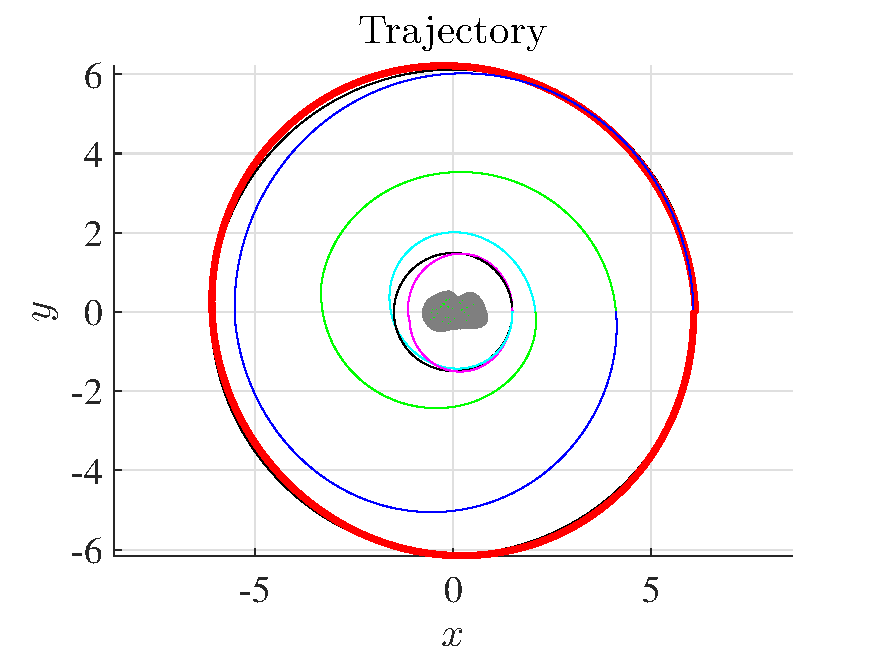
\includegraphics[width=\textwidth]{figures/trajectory.pdf}
        \caption{Equatorial view of transfer} \label{fig:trajectory_up} 
    \end{subfigure}~
    \begin{subfigure}[htbp]{0.45\textwidth} 
        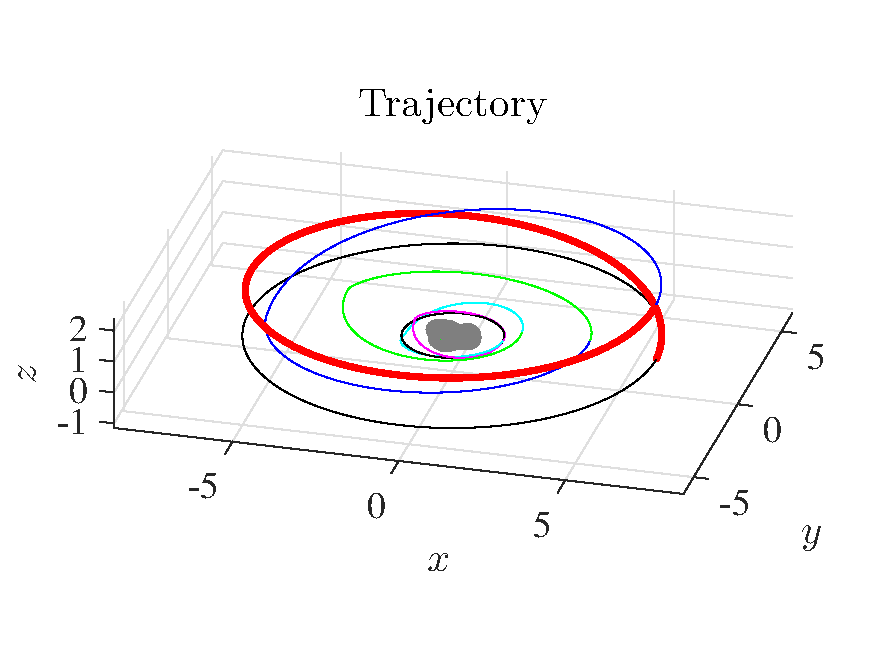
\includegraphics[width=\textwidth]{figures/trajectory_3d.pdf} 
        \caption{Out of plane view} \label{fig:trajectory_3d} 
    \end{subfigure}~ 
    \caption{Complete transfer trajectory}
    \label{fig:trajectory} 
\end{figure}

\subsection{Polyhedron Potential Model}\label{sec:polyhedron_potential}

% most use a spherical harmonic model or a ellipsoid model but we use a polyhedron model
An accurate gravitational potential model is necessary for the operation of spacecraft about asteroids.
Additionally, a detailed shape model of the asteroid is needed for trajectories passing close to the body.
The classic approach is to expand the gravitational potential into a harmonic series and compute the series coefficients.
However, the harmonic expansion is always an approximation as a result of the infinite order series used in the representation.
Additionally, the harmonic model used outside of the circumscribing sphere is not guaranteed to converge inside the sphere, which makes it unsuitable for trajectories near the surface.

We represent the gravitational potential of the asteroid using a polyhedron gravitation model.
This model is composed of a polyhedron, which is a three-dimensional solid body, that is defined by a series of vectors in the body-fixed frame.
The vectors define vertices in the body-fixed frame as well as planar faces which compose the surface of the asteroid.
We assume that each face is a triangle composed of three vertices and three edges.
As a result, only two faces meet at each edge while three faces meet at each vertex.
Only the body-fixed vectors, and their associated topology, is required to define the exterior gravitational model.
References~\citenum{werner1994} and~\citenum{werner1996} give a detailed derivation of the polyhedron model.
Here, we summarize the key developments and equations required for implementation.

Consider three vectors \( \vecbf{v}_1, \vecbf{v}_2, \vecbf{v}_3 \in \R^{3 \times 1} \), assumed to be ordered in a counterclockwise direction about an outward facing normal vector, which define a face.
It is easy to define the three edges of each face as
\begin{align}\label{eq:edges}
    \vecbf{e}_{i+1,i} = \vecbf{v}_{i+1} - \vecbf{v}_i \in \R^{3 \times 1 },
\end{align}
where the index \( i \in \parenth{1,2,3} \) is used to permute all edges of each face.
Since each edge is a member of two faces, there exist two edges which are defined in opposite directions between the same vertices.
We can also define the outward normal vector to face \( f\)  as
\begin{align}\label{eq:face_normal}
    \hat{\vecbf{n}}_f &= \parenth{\vecbf{v}_{2} - \vecbf{v}_1} \times \parenth{\vecbf{v}_{3} - \vecbf{v}_2} \in \R^{3 \times 1},
\end{align}
and the outward facing normal vector to each edge as
\begin{align}\label{eq:edge_normal}
    \hat{\vecbf{n}}_{i+1,i}^f &= \parenth{\vecbf{v}_{i+1} - \vecbf{v}_i} \times \hat{\vecbf{n}}_f \in \R^{3 \times 1}.
\end{align}
For each face we define the face dyad \( \vecbf{F}_f \) as
\begin{align}\label{eq:face_dyad}
    \vecbf{F}_f &= \hat{\vecbf{n}}_f \hat{\vecbf{n}}_f \in \R^{3 \times 3}.
\end{align}
Each edge is a member of two faces and has an outward pointing edge normal vector, given in~\cref{eq:edge_normal}, perpendicular to both the edge and the face normal.
For the edge connecting the vectors \( \vecbf{v}_1 \) and \( \vecbf{v}_2 \), which are shared between the faces \(A\) and \( B\), the per edge dyad is given by
\begin{align}\label{eq:edge_dyad}
    \vecbf{E}_{12} = \hat{\vecbf{n}}_A \hat{\vecbf{n}}_{12}^A + \hat{\vecbf{n}}_B \hat{\vecbf{n}}_{21}^B \in \R^{3 \times 3}.
\end{align}
The edge dyad \( \vecbf{E}_e  \), is defined for each edge and is a function of the two adjacent faces meeting at that edge.
The face dyad \( \vecbf{F}_f \), is defined for each face and is a function of the face normal vectors.

Let \( \vecbf{r}_i \in \R^{3 \times 1} \) be the vector from the spacecraft to the vertex \( \vecbf{v}_i \) and it's length is given by \( r_i = \norm{\vecbf{r}_i} \in \R^{1} \).
The per-edge factor \( L_e \in \R^{1}\), for the edge connecting vertices \( \vecbf{v}_i \) and \( \vecbf{v}_j \), with a constant length \( e_{ij} = \norm{\vecbf{e}_{ij}} \in \R^1\) is
\begin{align}\label{eq:edge_factor}
    L_e &= \ln \frac{r_i + r_j + e_{ij}}{r_i + r_j - e_{ij}}.
\end{align}
For the face defined by the vertices \( \vecbf{v}_i, \vecbf{v}_j, \vecbf{v}_k \) the per-face factor \( \omega_f \in \R^{1} \) is
\begin{align}\label{eq:face_factor}
    \omega_f &= 2 \arctan \frac{\vecbf{r}_i \cdot \vecbf{r}_j \times \vecbf{r}_k}{r_i r_j r_k + r_i \parenth{\vecbf{r}_j \cdot \vecbf{r}_k} + r_j \parenth{\vecbf{r}_k \cdot \vecbf{r}_i} + r_k \parenth{\vecbf{r}_i \cdot \vecbf{r}_j}} .
\end{align}
The gravitational potential due to a constant density polyhedron is given as
\begin{align}\label{eq:potential}
    U(\vecbf{r}) &= \frac{1}{2} G \sigma \sum_{e \in \text{edges}} \vecbf{r}_e \cdot \vecbf{E}_e \cdot \vecbf{r}_e \cdot L_e - \frac{1}{2}G \sigma \sum_{f \in \text{faces}} \vecbf{r}_f \cdot \vecbf{F}_f \cdot \vecbf{r}_f \cdot \omega_f \in \R^1,
\end{align}
where \( \vecbf{r}_e\) and \(\vecbf{r}_f \) are the vectors from the spacecraft to any point on the respective edge or face, \( G\) is the universal gravitational constant, and \( \sigma \) is the constant density of the asteroid.
Furthermore we can use these definitions to define the attraction, gravity gradient matrix, and Laplacian as
\begin{align}
    \nabla U ( \vecbf{r} ) &= -G \sigma \sum_{e \in \text{edges}} \vecbf{E}_e \cdot \vecbf{r}_e \cdot L_e + G \sigma \sum_{f \in \text{faces}} \vecbf{F}_f \cdot \vecbf{r}_f \cdot \omega_f \in \R^{3 \times 1} , \label{eq:attraction}\\
    \nabla \nabla U ( \vecbf{r} ) &= G \sigma \sum_{e \in \text{edges}} \vecbf{E}_e  \cdot L_e - G \sigma \sum_{f \in \text{faces}} \vecbf{F}_f \cdot \omega_f \in \R^{3 \times 3}, \label{eq:gradient_matrix}\\
    \nabla^2 U &= -G \sigma \sum_{f \in \text{faces}}  \omega_f \in \R^1 .\label{eq:laplacian}
\end{align}

One interesting thing to note is that both~\cref{eq:face_dyad,eq:edge_dyad} can be precomputed without knowledge of the position of the satellite.
They are both solely functions of the vertices and edges of the polyhedral shape model and are computed once and stored.
Once a position vector \( \vecbf{r} \) is defined, the scalars given in~\cref{eq:edge_factor,eq:face_factor} can be computed for each face and edge.
Finally,~\cref{eq:potential} is used to compute the gravitational potential on the spacecraft.
The Laplacian, defined in~\cref{eq:laplacian}, gives a simple method to determine if the spacecraft has collided with the body~\cite{werner1996}. 

\subsection{Itokawa Shape Model and Simulated Imagery}\label{sec:imagery}
In this work, we consider trajectories about asteroid Itokawa.
Itokawa was the target of the Hayabusa mission and detailed shape and surface maps have been generated~\cite{kawaguchi2006,tanimoto2013}.
We use the estimated rotation period of \SI{12.1}{\hour} with a nominal density of \SI{1.9}{\gram\per\centi\meter\cubed}~\cite{fujiwara2006}.
% TODO: look up how many facets in the itokawa high model
The shape model is composed of \num{4092} triangular faces and a rendering of the asteroid is provided in~\cref{fig:itokawa_3d}.
A highly detailed model is used to for the shape of the asteroid to provide a more detailed and feature rich imaging target. 
However, the polyhedron potential model uses a much coarser shape composed of \num{64} faces. 
This greatly reduces the complexity of the potential model without a significant difference in the qualitative nature of the dynamic environment.
% TODO: Insert a picture of Itokawa generated from Blender. Use the high quality model

% TODO: Add some detail on Blender and image processing
\begin{itemize}
    \item Simulate images using blender
    \item Discuss some basics of visual odometry and feature detection
\end{itemize}    
\section{Nonlinear Landing Controller on \SE}\label{sec:controller}

% TODO: detail on nonlinear controller
\begin{itemize}
    \item Show development of \SE controller
    \item Summarize the stability proof for trajectory tracking
    \item We're assuming a fully actuated spacecraft
\end{itemize}


A wide variety of control schemes have been proposed for asteroid landing missions~\cite{furfaro2013,li2011a}.
In addition, there are a  variety of controllers developed for systems evolving on \( \SE \)~\cite{lee2010c, goodarzi2015}.
In this paper, we extend their use from quadrotor aerial vehicles into the space domain. 
This approach addresses many of the issues associated with the previous work on asteroid landings.

The geometric control methods used to develop these nonlinear controllers allow for the development of control systems for dynamic systems which evolve on nonlinear manifolds. 
By developing the control system directly on the nonlinear manifold, geometric control techniques provide unique advantages as compared to those developed using local coordinate representations.
Furthermore, the geometric controller avoids the chattering issues inherent in the previous sliding mode control approaches to asteroid landing.
In addition, rather than offering only a bounded stability guarantee, the proposed nonlinear geometric controller guarantees almost global tracking of the attitude and translational states. 
This stability guarantee is critical for mission operations passing close to the surface over highly irregular terrain.
Furthermore, the coupled geometric controller explicitly considers the attitude coupling of the body in contrast to many of the previous approaches.

\section{Numerical Simulation}\label{sec:simulation}

% TODO: Itokawa simulation
\begin{itemize}
    \item Simulation about asteroid Itokawa
    \item Using Blender for generating simulated imagery
    \item Describe the body fixed vertical descent (straight vertical descent in body frame)
    \item how to determine attitude trajectory to ensure spacecraft points at asteroid
\end{itemize}

\section{Conclusions}\label{sec:conclusions}
There have been a variety of approaches for the analysis and design of orbital trajectories around asteroids.
Relatively less work has been directed towards the design of landing trajectories.
Furthermore, much of the previous work has only treated the orbital or translational dynamics.
The approximation of a spacecraft as a point mass rather than an extended rigid body severely limits the applicability and ignores a major component of the dynamic environment.
This work directly derives the equations of motion of a dumbbell spacecraft around an asteroid described using a polyhedron potential model. 
We explicitly consider the impact of the gravitational moment on both the orbit and attitude dynamics. 
With this accurate equations of motion we develop geometric nonlinear controllers which allow for the vehicle to track a desired landing trajectory. 
The landing portion allows for an end to end mission design scheme based on rigorous geometric mechanics techniques.

\bibliographystyle{AAS_publication} 
\bibliography{library}

\end{document}
